\documentclass{article}

% if you need to pass options to natbib, use, e.g.:
% \PassOptionsToPackage{numbers, compress}{natbib}
% before loading nips_2018

% ready for submission
% \usepackage{nips_2018}

% to compile a preprint version, e.g., for submission to arXiv, add
% add the [preprint] option:
\usepackage[preprint]{nips_2018}

% to compile a camera-ready version, add the [final] option, e.g.:
% \usepackage[final]{nips_2018}

% to avoid loading the natbib package, add option nonatbib:
% \usepackage[nonatbib]{nips_2018}

\usepackage[utf8]{inputenc} % allow utf-8 input
\usepackage[T1]{fontenc}    % use 8-bit T1 fonts
\usepackage{hyperref}       % hyperlinks
\usepackage{url}            % simple URL typesetting
\usepackage{booktabs}       % professional-quality tables
\usepackage{amsfonts}       % blackboard math symbols
\usepackage{nicefrac}       % compact symbols for 1/2, etc.
\usepackage{microtype}      % microtypography
\usepackage{caption}
\usepackage{todo}
\usepackage{graphicx}
\graphicspath{ {./graphics/} }

\title{ %Towards Higher Capacity, Regularized Models: 
  Solving OpenAI's
  Car Racing Environment with Deep Reinforcement Learning and Dropout} 

%% The \author macro works with any number of authors. There are two
%% commands used to separate the names and addresses of multiple
%% authors: \And and \AND.

%% Using \And between authors leaves it to LaTeX to determine where to
%% break the lines. Using \AND forces a line break at that point. So,
%% if LaTeX puts 3 of 4 authors names on the first line, and the last
%% on the second line, try using \AND instead of \And before the third
%% author name.
\newcommand*\samethanks[1][\value{footnote}]{\footnotemark[#1]}
\author{
  Patrik Gerber\thanks{Denotes equal contribution to this work.}\\
  University of Oxford \\
  % \texttt{patrik.gerber@ccc.ox.ac.uk} \\
  \And
  Jiajing Guan\samethanks \\
  George Mason University \\ 
  % \texttt{jiajingguan@gmail.com} \\
  \And
  Elvis Nunez\samethanks \\
  Brown University \\
  % \texttt{elvis@brown.io} \\
  \And
  Kaman Phamdo\samethanks \\
  University of Maryland \\
  % \texttt{kaman@phamdo.com} \\
  \And
  Tonmoy Monsoor \\
  University of California, Los Angeles \\
  % \texttt{mtonmoy@g.ucla.edu} \\
  \And
  Nicholas Malaya \\ % typically, supervisor is last author
  AMD Research \\ 
  % \texttt{nicholas.malaya@amd.com} \\
}

\begin{document}
% \nipsfinalcopy is no longer used

\maketitle

\begin{abstract}

%% key points addressed in paper: 
  
%% Since decision making is hard under partial observability do we want
%% to use more complex models and solve them approximately or use
%% (inaccurate) simple models and solve them exactly?  

%% How can we extend deep RL methods to robustly solve partially
%% observable problems? 

%% Can we learn concise abstractions of history that are sufficient for
%% high-quality decision-making? 
  
%Deep Reinforcement Learning methods have seen many successes in recent
%years, ranging from solving classical video games to beating world
  %class Go players.
Reinforcement Learning models are typically trained for
narrow, well-defined tasks. They perform well in their defined task,
but changes in the environment often cause disproportionate reductions
in performance. In this paper, an example which suggests that
regularization methods could improve the generalization capacity of
deep RL algorithms is provided. 
This is explored in OpenAI’s Car Racing environment where the agent
observes only a small subset of the state space during training.
%by
%applying the DDQN-algorithm with dropout. 
\end{abstract}

\vspace{-4mm}
\section{Introduction}
Deep reinforcement learning methods have proven successful in solving
well-defined computer
games\cite{mnih2013playing,silver2017mastering,zambaldi2018relational,bansal2017emergent}. 
However, deep RL agents are limited by their sensitivity
to perturbations in the environment. They can fail catastrophically
when applied to environments that differ even slightly from where they
were trained\cite{kansky2017schema,taylor2009transfer}. This indicates
the models are not generalizing well, have overfit to prior
experiences, and are not likely to transfer to other tasks
effectively\cite{dibangoye2018learning}. 

In this paper, a deep RL algorithm that uses dropout
\cite{Dropout} is used to successfully solve the game of
CarRacing-v0\cite{CarRacing}. The model is trained on a
limited state space made up of 3 tracks used as a form of curriculum
learning\cite{bengio2009curriculum}. This result shows that
regularization methods such as dropout can mitigate the overfit
usually exhibited by deep RL. This task is particularly challenging
because the track is randomly generated for each game. The environment
has recently been solved using a generative network, but previous
attempts using deep RL methods have not been successful
\cite{World_Models} \cite{CarRacing1}. It is believed this solution is
the first to solve the challenge using deep RL.  

%\section{Methods}
The DDQN algorithm \cite{DQN,DDQN} was used.
Following the original DQN algorithm \cite{DQN}, the architecture
for the Q-network consists of 3 convolutional layers followed by 2
dense layers and an output for each of the five actions.
This is compared with a modified version, where a dropout layer is
added to the second convolutional layer to regularize the model.  
The models were trained with varying observability of the
environment. The experiments were performed on three different subsets of
the state space: a single fixed racetrack, three fixed racetracks, and 
randomly generated racetracks. The models were then tested on 100
random tracks.
%, generated from random seeds $1$ through $100$. 

\begin{figure}[!h]
\captionsetup{justification=centering}
\centering
\begin{minipage}[t]{.3\textwidth}
  \centering
  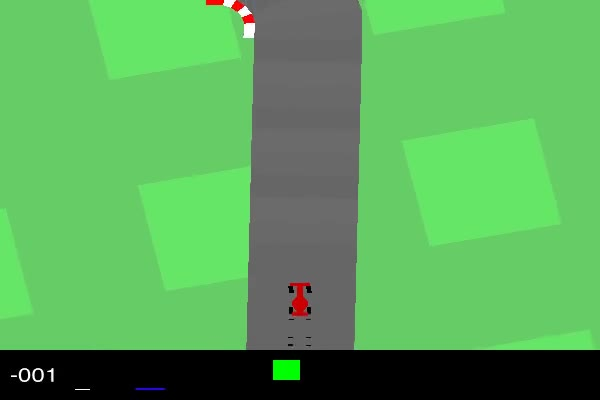
\includegraphics[width=\linewidth]{Graphics/carracing.jpg}
  \caption{CarRacing-v0 environment. The red car's score increases as
    it traverses cells colored grey, and is decreased when leaving the
  track (green cells).}
  \label{fig:curves_comparison}
\end{minipage}
\hspace{.25cm}
\begin{minipage}[t]{.3\textwidth}
  \centering
  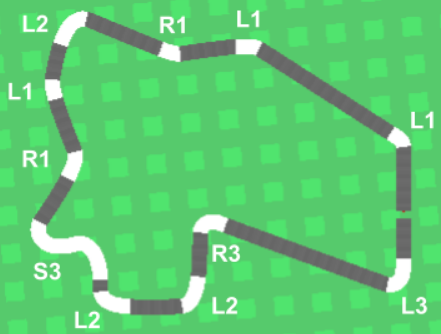
\includegraphics[width=\linewidth]{Graphics/curves.png}
  \caption{A full track, with each corner labelled by the different
    types of curves.} 
  \label{fig:curves}
\end{minipage}
\hspace{.25cm}
\begin{minipage}[t]{.32\textwidth}
  \centering
  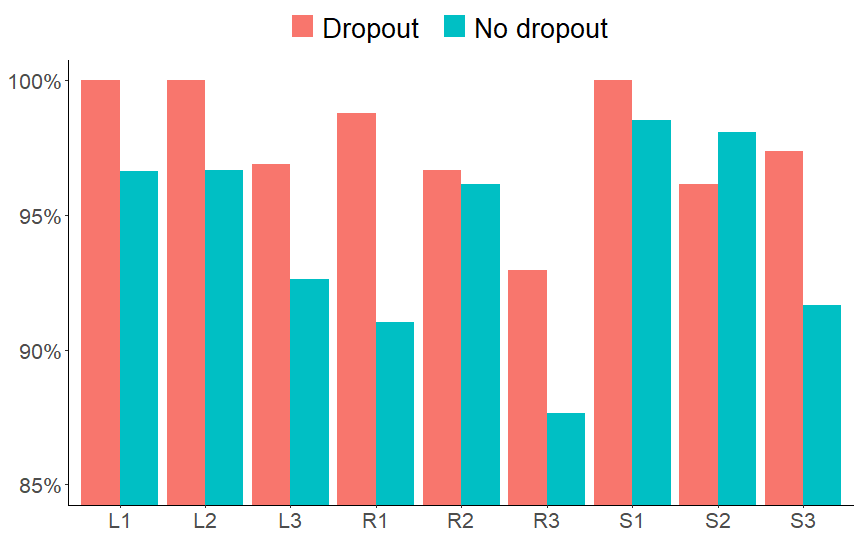
\includegraphics[width=\linewidth]{Graphics/curve_plot_v2.png}
  \caption{Proportion of tiles visited on different curves. The grey
    bars are the general DDQN network, and the black bars are the
    network with the inclusion of a dropout layer. In each case the
    accuracy improves with dropout.} 
%  \caption{Different types of curves. }
  \label{fig:curves_comparison}
\end{minipage}
\vspace{-2.5mm}
\end{figure}


%% \begin{figure}[!h]
%% \captionsetup{justification=centering}
%% \centering
%% 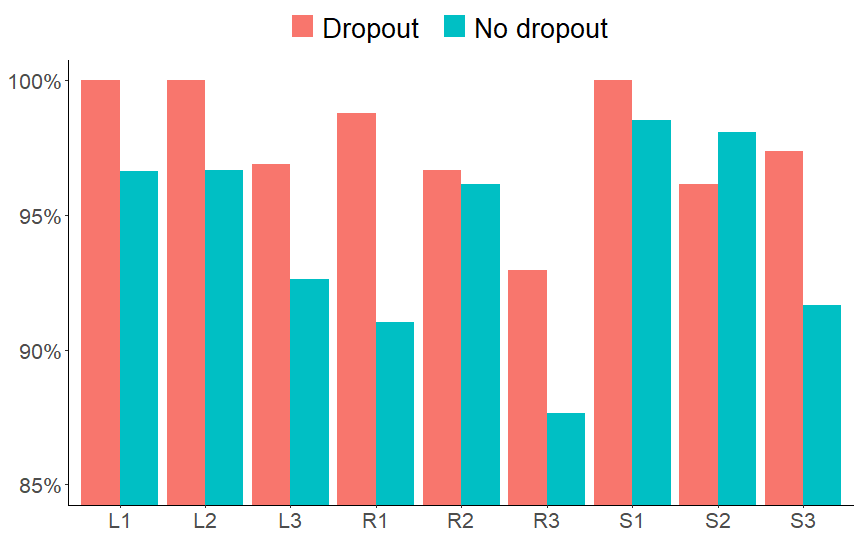
\includegraphics[width=.55\linewidth]{Graphics/curve_plot_v2.png}
%% \caption{Proportion of tiles visited on different curves. }
%% \label{fig:curves_comparison}
%% \vspace{-4mm}
%% \end{figure}


\section{Performance Analysis}
As shown in Tables \ref{tab:base_scores} and \ref{tab:drop_scores},
the average scores over 100 random games improved in all three
environments when dropout was applied to the Q-network. To
investigate the generalization capacity of these models, a curve 
classification algorithm was developed. Each curve in the racetrack is
charactertized as either a Left, Right, or S-shaped curve. Then, the
steepness of the curve is ranked from 1 to 3, where 1 represents a
shallow curve and 3 represents a steep curve. 
For each of these different types of curves, the percentage
of tiles cleared is used as a metric of the car's performance. 
The proportion of tiles visited for each curve over 100 tracks is
shown in Figure~\ref{fig:curves_comparison}. Dropout serves to
improve the car's performance through each curve, with particularly
large improvements in L3, R3, and S3, the steepest curves
encountered. These steep curves are the least common curve encountered
in the training data. It is possible that unregularized models are not
accurately adapting to these curves, and are overfitting to the more
common (and shallower) curves. This can be catastrophic, as a sharp
turn requires less velocity or the car will leave the track. In
addition to a higher average score, notice also that the standard
deviation of scores substantially  decreased in the cases using
dropout. Observations indicate that this reduction in variation was
because of fewer catastrophic crashes of the car in the cases
regularized with dropout.  

\begin{table}[h!]
\begin{center}
\begin{minipage}[t]{.4\textwidth}
  \begin{tabular}{c|c}
    \textbf{Environment} & \textbf{Average Score}\\ \hline
    1 Fixed Track & $849.99\pm78.72$ \\
    3 Fixed Tracks & $853.88\pm127.71$ \\
    Random Tracks & $854.83\pm107.14$ \\
  \end{tabular}
  \caption{Performance without dropout}
  \label{tab:base_scores}
\end{minipage}
\hspace{1cm}
\begin{minipage}[t]{.4\textwidth}
  \begin{tabular}{c|c}
    \textbf{Environment} & \textbf{Average Score}\\
    \hline
    1 Fixed Track & $894.38\pm24.5$ \\
    \bf{3 Fixed Tracks} & \bf{$906.67\pm23.6$} \\
    Random Tracks & $892.62\pm41.48$ \\
  \end{tabular}
  \caption{Performance with dropout. The game winning result is shown
    in bold. }
  \label{tab:drop_scores}
\end{minipage}
\end{center}
\vspace{-5mm}
\end{table}

Figure \ref{fig:curves_comparison} compares the performance of the
models trained on a single racetrack. Even though both models were
trained on the same racetrack, the model with dropout performed better
than the model without dropout, especially on curves that the agent
did not see examples of during training. This indicates that 
dropout is an effective regularizer and is improving the
generalization of the model. 

\section{Conclusions and Future Work}
A deep RL solution was shown to solve CarRacing-v0 where the agent was
trained on just three fixed racetracks. 
Regularization improved the algorithm's ability to generalize to
situations not observed during training. These results suggest
that common regularization techniques such as dropout can be
applied successfully to improve robustness and generalization capacity
of deep RL algorithms. This is especially fruitful in applications
particularly prone to overfitting, such as environments where the
agent has access to only a subset of the state space during training.
Higher capacity networks may change the balance between optimal
parallelization of RL tasks between CPUs and GPUs\cite{stooke2018accelerated}. 

These results are preliminary, and are only shown for the CarRacing-v0
environment. Future work will focus on extending these methods to
additional environments. Particular focus will be on changing
parameters of the enviroment that the model had little or no training
data on, to observe the generalization capacity in these cases. 

% -------------------------------------------------------------------------------------------------------------------
% -------------------------------------------------------------------------------------------------------------------
% -------------------------------------------------------------------------------------------------------------------
% -------------------------------------------------------------------------------------------------------------------
% -------------------------------------------------------------------------------------------------------------------
% -------------------------------------------------------------------------------------------------------------------
% -------------------------------------------------------------------------------------------------------------------


% \section{Submission of papers to NIPS 2018}

% NIPS requires electronic submissions.  The electronic submission site
% is
% \begin{center}
%   \url{https://cmt.research.microsoft.com/NIPS2018/}
% \end{center}

% Please read the instructions below carefully and follow them faithfully.

% \subsection{Style}

% Papers to be submitted to NIPS 2018 must be prepared according to the
% instructions presented here. Papers may only be up to eight pages
% long, including figures. Additional pages \emph{containing only
%   acknowledgments and/or cited references} are allowed. Papers that
% exceed eight pages of content (ignoring references) will not be
% reviewed, or in any other way considered for presentation at the
% conference.

% The margins in 2018 are the same as since 2007, which allow for
% $\sim$$15\%$ more words in the paper compared to earlier years.

% Authors are required to use the NIPS \LaTeX{} style files obtainable
% at the NIPS website as indicated below. Please make sure you use the
% current files and not previous versions. Tweaking the style files may
% be grounds for rejection.

% \subsection{Retrieval of style files}

% The style files for NIPS and other conference information are
% available on the World Wide Web at
% \begin{center}
%   \url{http://www.nips.cc/}
% \end{center}
% The file \verb+nips_2018.pdf+ contains these instructions and
% illustrates the various formatting requirements your NIPS paper must
% satisfy.

% The only supported style file for NIPS 2018 is \verb+nips_2018.sty+,
% rewritten for \LaTeXe{}.  \textbf{Previous style files for \LaTeX{}
%   2.09, Microsoft Word, and RTF are no longer supported!}

% The \LaTeX{} style file contains three optional arguments: \verb+final+,
% which creates a camera-ready copy, \verb+preprint+, which creates a
% preprint for submission to, e.g., arXiv, and \verb+nonatbib+, which will
% not load the \verb+natbib+ package for you in case of package clash.

% \paragraph{New preprint option for 2018}
% If you wish to post a preprint of your work online, e.g., on arXiv,
% using the NIPS style, please use the \verb+preprint+ option. This will
% create a nonanonymized version of your work with the text
% ``Preprint. Work in progress.''  in the footer. This version may be
% distributed as you see fit. Please \textbf{do not} use the
% \verb+final+ option, which should \textbf{only} be used for papers
% accepted to NIPS.

% At submission time, please omit the \verb+final+ and \verb+preprint+
% options. This will anonymize your submission and add line numbers to aid
% review. Please do \emph{not} refer to these line numbers in your paper
% as they will be removed during generation of camera-ready copies.

% The file \verb+nips_2018.tex+ may be used as a ``shell'' for writing
% your paper. All you have to do is replace the author, title, abstract,
% and text of the paper with your own.

% The formatting instructions contained in these style files are
% summarized in Sections \ref{gen_inst}, \ref{headings}, and
% \ref{others} below.

% \section{General formatting instructions}
% \label{gen_inst}

% The text must be confined within a rectangle 5.5~inches (33~picas)
% wide and 9~inches (54~picas) long. The left margin is 1.5~inch
% (9~picas).  Use 10~point type with a vertical spacing (leading) of
% 11~points.  Times New Roman is the preferred typeface throughout, and
% will be selected for you by default.  Paragraphs are separated by
% \nicefrac{1}{2}~line space (5.5 points), with no indentation.

% The paper title should be 17~point, initial caps/lower case, bold,
% centered between two horizontal rules. The top rule should be 4~points
% thick and the bottom rule should be 1~point thick. Allow
% \nicefrac{1}{4}~inch space above and below the title to rules. All
% pages should start at 1~inch (6~picas) from the top of the page.

% For the final version, authors' names are set in boldface, and each
% name is centered above the corresponding address. The lead author's
% name is to be listed first (left-most), and the co-authors' names (if
% different address) are set to follow. If there is only one co-author,
% list both author and co-author side by side.

% Please pay special attention to the instructions in Section \ref{others}
% regarding figures, tables, acknowledgments, and references.

% \section{Headings: first level}
% \label{headings}

% All headings should be lower case (except for first word and proper
% nouns), flush left, and bold.

% First-level headings should be in 12-point type.

% \subsection{Headings: second level}

% Second-level headings should be in 10-point type.

% \subsubsection{Headings: third level}

% Third-level headings should be in 10-point type.

% \paragraph{Paragraphs}

% There is also a \verb+\paragraph+ command available, which sets the
% heading in bold, flush left, and inline with the text, with the
% heading followed by 1\,em of space.

% \section{Citations, figures, tables, references}
% \label{others}

% These instructions apply to everyone.

% \subsection{Citations within the text}

% The \verb+natbib+ package will be loaded for you by default.
% Citations may be author/year or numeric, as long as you maintain
% internal consistency.  As to the format of the references themselves,
% any style is acceptable as long as it is used consistently.

% The documentation for \verb+natbib+ may be found at
% \begin{center}
%   \url{http://mirrors.ctan.org/macros/latex/contrib/natbib/natnotes.pdf}
% \end{center}
% Of note is the command \verb+\citet+, which produces citations
% appropriate for use in inline text.  For example,
% \begin{verbatim}
%    \citet{hasselmo} investigated\dots
% \end{verbatim}
% produces
% \begin{quote}
%   Hasselmo, et al.\ (1995) investigated\dots
% \end{quote}

% If you wish to load the \verb+natbib+ package with options, you may
% add the following before loading the \verb+nips_2018+ package:
% \begin{verbatim}
%    \PassOptionsToPackage{options}{natbib}
% \end{verbatim}

% If \verb+natbib+ clashes with another package you load, you can add
% the optional argument \verb+nonatbib+ when loading the style file:
% \begin{verbatim}
%    \usepackage[nonatbib]{nips_2018}
% \end{verbatim}

% As submission is double blind, refer to your own published work in the
% third person. That is, use ``In the previous work of Jones et
% al.\ [4],'' not ``In our previous work [4].'' If you cite your other
% papers that are not widely available (e.g., a journal paper under
% review), use anonymous author names in the citation, e.g., an author
% of the form ``A.\ Anonymous.''

% \subsection{Footnotes}

% Footnotes should be used sparingly.  If you do require a footnote,
% indicate footnotes with a number\footnote{Sample of the first
%   footnote.} in the text. Place the footnotes at the bottom of the
% page on which they appear.  Precede the footnote with a horizontal
% rule of 2~inches (12~picas).

% Note that footnotes are properly typeset \emph{after} punctuation
% marks.\footnote{As in this example.}

% \subsection{Figures}

% \begin{figure}
%   \centering
%   \fbox{\rule[-.5cm]{0cm}{4cm} \rule[-.5cm]{4cm}{0cm}}
%   \caption{Sample figure caption.}
% \end{figure}

% All artwork must be neat, clean, and legible. Lines should be dark
% enough for purposes of reproduction. The figure number and caption
% always appear after the figure. Place one line space before the figure
% caption and one line space after the figure. The figure caption should
% be lower case (except for first word and proper nouns); figures are
% numbered consecutively.

% You may use color figures.  However, it is best for the figure
% captions and the paper body to be legible if the paper is printed in
% either black/white or in color.

% \subsection{Tables}

% All tables must be centered, neat, clean and legible.  The table
% number and title always appear before the table.  See
% Table~\ref{sample-table}.

% Place one line space before the table title, one line space after the
% table title, and one line space after the table. The table title must
% be lower case (except for first word and proper nouns); tables are
% numbered consecutively.

% Note that publication-quality tables \emph{do not contain vertical
%   rules.} Strongly suggest the use of the \verb+booktabs+ package,
% which allows for typesetting high-quality, professional tables:
% \begin{center}
%   \url{https://www.ctan.org/pkg/booktabs}
% \end{center}
% This package was used to typeset Table~\ref{sample-table}.

% \begin{table}
%   \caption{Sample table title}
%   \label{sample-table}
%   \centering
%   \begin{tabular}{lll}
%     \toprule
%     \multicolumn{2}{c}{Part}                   \\
%     \cmidrule(r){1-2}
%     Name     & Description     & Size ($\mu$m) \\
%     \midrule
%     Dendrite & Input terminal  & $\sim$100     \\
%     Axon     & Output terminal & $\sim$10      \\
%     Soma     & Cell body       & up to $10^6$  \\
%     \bottomrule
%   \end{tabular}
% \end{table}

% \section{Final instructions}

% Do not change any aspects of the formatting parameters in the style
% files.  In particular, do not modify the width or length of the
% rectangle the text should fit into, and do not change font sizes
% (except perhaps in the \textbf{References} section; see below). Please
% note that pages should be numbered.

% \section{Preparing PDF files}

% Please prepare submission files with paper size ``US Letter,'' and
% not, for example, ``A4.''

% Fonts were the main cause of problems in the past years. Your PDF file
% must only contain Type 1 or Embedded TrueType fonts. Here are a few
% instructions to achieve this.

% \begin{itemize}

% \item You should directly generate PDF files using \verb+pdflatex+.

% \item You can check which fonts a PDF files uses.  In Acrobat Reader,
%   select the menu Files$>$Document Properties$>$Fonts and select Show
%   All Fonts. You can also use the program \verb+pdffonts+ which comes
%   with \verb+xpdf+ and is available out-of-the-box on most Linux
%   machines.

% \item The IEEE has recommendations for generating PDF files whose
%   fonts are also acceptable for NIPS. Please see
%   \url{http://www.emfield.org/icuwb2010/downloads/IEEE-PDF-SpecV32.pdf}

% \item \verb+xfig+ "patterned" shapes are implemented with bitmap
%   fonts.  Use "solid" shapes instead.

% \item The \verb+\bbold+ package almost always uses bitmap fonts.  You
%   should use the equivalent AMS Fonts:
% \begin{verbatim}
%    \usepackage{amsfonts}
% \end{verbatim}
% followed by, e.g., \verb+\mathbb{R}+, \verb+\mathbb{N}+, or
% \verb+\mathbb{C}+ for $\mathbb{R}$, $\mathbb{N}$ or $\mathbb{C}$.  You
% can also use the following workaround for reals, natural and complex:
% \begin{verbatim}
%    \newcommand{\RR}{I\!\!R} %real numbers
%    \newcommand{\Nat}{I\!\!N} %natural numbers
%    \newcommand{\CC}{I\!\!\!\!C} %complex numbers
% \end{verbatim}
% Note that \verb+amsfonts+ is automatically loaded by the
% \verb+amssymb+ package.

% \end{itemize}

% If your file contains type 3 fonts or non embedded TrueType fonts, 
% will ask you to fix it.

% \subsection{Margins in \LaTeX{}}

% Most of the margin problems come from figures positioned by hand using
% \verb+\special+ or other commands. Suggest using the command
% \verb+\includegraphics+ from the \verb+graphicx+ package. Always
% specify the figure width as a multiple of the line width as in the
% example below:
% \begin{verbatim}
%    \usepackage[pdftex]{graphicx} ...
%    \includegraphics[width=0.8\linewidth]{myfile.pdf}
% \end{verbatim}
% See Section 4.4 in the graphics bundle documentation
% (\url{http://mirrors.ctan.org/macros/latex/required/graphics/grfguide.pdf})

% A number of width problems arise when \LaTeX{} cannot properly
% hyphenate a line. Please give LaTeX hyphenation hints using the
% \verb+\-+ command when necessary.

% \subsubsection*{Acknowledgments}

% Use unnumbered third level headings for the acknowledgments. All
% acknowledgments go at the end of the paper. Do not include
% acknowledgments in the anonymized submission, only in the final paper.

% -------------------------------------------------------------------------------------------------------------------
% -------------------------------------------------------------------------------------------------------------------
% -------------------------------------------------------------------------------------------------------------------
% -------------------------------------------------------------------------------------------------------------------
% -------------------------------------------------------------------------------------------------------------------
% -------------------------------------------------------------------------------------------------------------------
% -------------------------------------------------------------------------------------------------------------------

\bibliographystyle{plain}
\bibliography{bibliography}

\section{Appendices}
\subsection{Car-Racing-v0}

OpenAI Gym’s CarRacing-v0 reinforcement learning testbed
\cite{CarRacing} is a is a top-down view car racing game where the
goal is to visit all tiles of the racetrack as quickly as
possible. The agent receives a reward of $-0.1$ at each time step and
$\frac{1000}{N}$ for each track tile visited, where $N$ is the total
number of tiles in the track. The state is represented by $96\times96$
RGB screenshots of the game. The game ends when the agent visits all
tiles on the track or when 1000 frames have passed. The environment is
considered solved by when the agent achieves an average score of 900
or above over 100 consecutive games. 


\subsection{Implementation}
The DDQN algorithm \cite{DDQN} was used. The input
to the Q-network is a $96\times96\times4$ tensor produced by stacking
4 consecutive frames of the game, and the output is five dimensional,
corresponding to the elements of the discretized action space. As
proposed in the original DQN algorithm \cite{DQN}, the architecture
for the Q-network consists of 3 convolutional layers followed by 2
dense layers and an output for each of the five actions. Each hidden
layer is followed by a rectified nonlinearity with dropout applied to
the second convolutional layer only. The model was trained over a
maximum of 3000 episodes corresponding to a training time of
approximately 36 hours, and early stopping was used to ensure that the
best performing model was selected for analysis.
%\todo{need stopping  criterion?}  

The best model was attained using three tracks as a form of curriculum
learning. These three tracks are shown below. 

\begin{figure}[!h]
\captionsetup{justification=centering}
\centering
\begin{minipage}[t]{.3\textwidth}
  \centering
  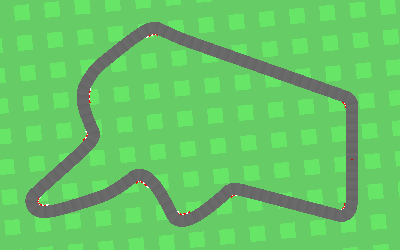
\includegraphics[width=\linewidth]{Graphics/track104.png}
  \caption{The first training track.}
  \label{fig:curves_comparison}
\end{minipage}
%\hspace{1cm}
\begin{minipage}[t]{.3\textwidth}
  \centering
  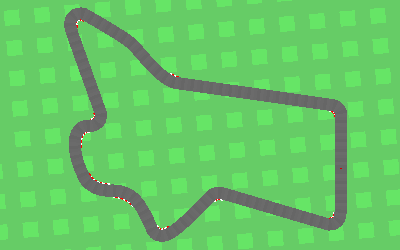
\includegraphics[width=\linewidth]{Graphics/track106.png}
  \caption{The second training track.}
  \label{fig:curves}
\end{minipage}
%\hspace{1cm}
\begin{minipage}[t]{.3\textwidth}
  \centering
  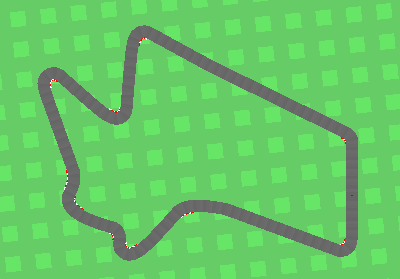
\includegraphics[width=\linewidth]{Graphics/track108.png}
  \caption{The third training track.}
  \label{fig:curves_comparison}
\end{minipage}
\vspace{-2.5mm}
\end{figure}

The code, implementated algorithm, and further model information can
be found at \url{https://github.com/AMD-RIPS/RL-2018}. A video of the
fully trained car running a track can be found at
\url{https://drive.google.com/file/d/1DQU4yCsq6nbVJB6WKoXlED9YFGDselIu/view}. 

\subsection{Network architecture}
See the table below for the exact architecture used in the models. 
\begin{table}[h!]
  \begin{center}
    \begin{tabular}{c|c|c}
      \textbf{Layer} & \textbf{Topology} & \textbf{Activation}\\
      \hline
      1 & Convolutional, 32 8x8 kernels with stride 4 & ReLU \\
      2 & Convolutional, 64 4x4 kernels with stride 2 & ReLU \\      
      3 & Convolutional, 64 3x3 kernels with stride 1 & ReLU \\
      4 & Dense, 512 neurons & ReLU \\
      output & Dense, 5 neurons & Linear \\
    \end{tabular}
    \vspace{0.1cm}
    \label{tab:network_architecture}
  \end{center}
\end{table}

\subsection{Action space}
The action space of OpenAI's CarRacing environment is the set $[-1,1]
\times [0,1]^2 \subset \mathbb{R}^3$. The space was discretized into
five possible actions. See the table below for more detail.  
\begin{table}[h!]
  \begin{center}
    \begin{tabular}{c|c}
      \textbf{Value} & \textbf{Interpretation} \\
      \hline
      $[-1,0,0]$ & Steer left \\
      $[1,0,0]$ & Steer right \\
      $[0,1,0]$ & Accelerate \\
      $[0,0,0.8]$ & Decelerate \\
      $[0,0,0]$ & Do nothing \\
    \end{tabular}
    \vspace{0.1cm}
    \label{tab:actions}
  \end{center}
\end{table}

\newpage
\subsection{Training parameters}
The table below details the training parameters that were used during
the training of the car-racing models.  
\begin{table}[h!]
  \begin{center}
    \begin{tabular}{c|c}
      \textbf{Parameter} & \textbf{Value} \\
      \hline
      Exploration rate & \begin{tabular}{@{}c@{}}Decrease from $1$ to
        $0.1$ linearly over \\ the first $250000$ frames, $0.1$
        thereafter\end{tabular} \\ 
      Optimizer & Default Tensorflow AdamOptimizer \\
      Learning rate & $0.00025$ \\
      Discount value & $0.99$ \\
      Batch size & $32$ \\
      Replay capacity & $100000$
    \end{tabular}
    \vspace{0.1cm}
    \label{tab:actions}
  \end{center}
\end{table}


\end{document}
